\documentclass[pdftex,letterpaper,12pt]{report}
\usepackage{thesis}
\usepackage{amsmath}
\usepackage{amssymb}
\usepackage{amsthm}
\usepackage{mathtools}
\usepackage{bm}
\usepackage{gensymb}
\usepackage{wasysym}
\usepackage{mathtools}
\usepackage{physics}
\usepackage{empheq}
\usepackage{cases}
\usepackage{rotating}
\usepackage{subfig}
\usepackage{caption}
\captionsetup{labelfont=bf} 
\captionsetup[subfloat]{position=top,singlelinecheck=off,justification=raggedright,font=bf,labelfont=large,labelformat=simple,captionskip=-2mm}
\usepackage{float}
\usepackage{enumitem} 
\usepackage[toc,page]{appendix}






\begin{document}
	
\begin{subequations}
	\begin{gather}
	\kappa_{0}^{Rb}=6.39+0.00914[T-200(^{\circ}C)]\\
	\kappa_{0}^{K}=5.99+0.0086[T-200(^{\circ}C)]\\
	\kappa_{0}^{Na}=4.84+0.00914[T-200(^{\circ}C)]
	\end{gather}
\end{subequations}

\begin{equation}
\kappa_{0}^{Rb-^{3}He}=4.52+0.00934[T(^{\circ}C)]
\end{equation}

$\Delta B \ll B$

\section{section}
\subsection{sub}
\subsubsection{sub1}
\subsubsection{sub2}

\begin{figure}[H]
	\centering
	\resizebox{0.91\textwidth}{!}{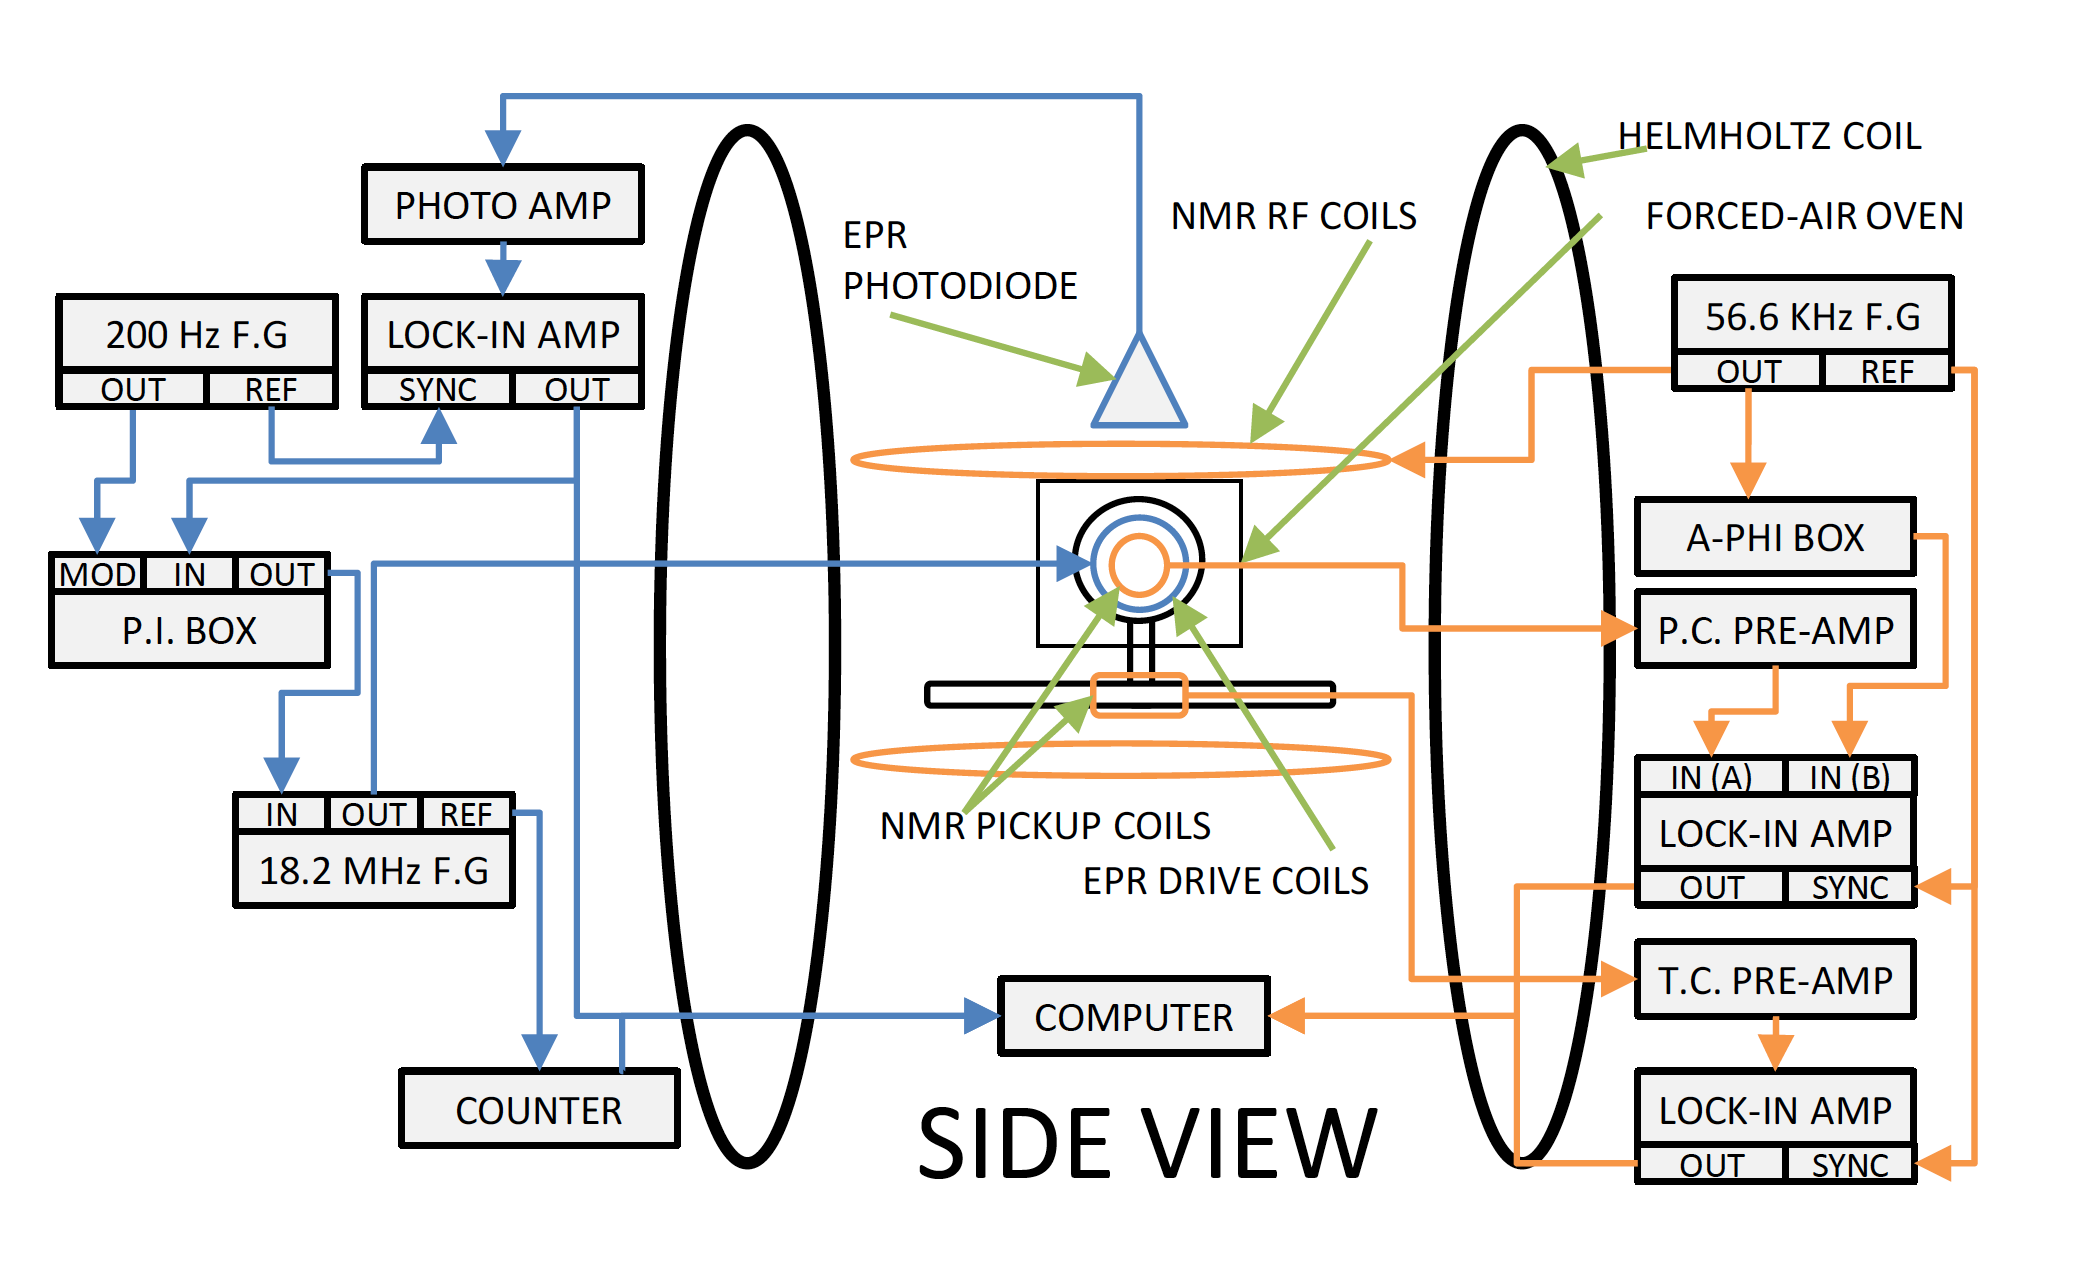
\includegraphics{AFPandEPRsetup.png}}
	\caption{{\bf EPR (left) and AFP (right) setup. Adapted from Dolph's PhD thesis.}}
	\label{AFPandEPRsetup}
\end{figure}

\emph{et al.}
5P$_{\frac{3}{2}}\rightarrow$

\addcontentsline{toc}{chapter}{Bibliography}
\bibliography{ref}

\end{document}